\documentclass[10pt, conference, compsocconf]{IEEEtran} %\documentclass[10pt, conference, compsocconf]{IEEEtran} %\documentclass[conference]{IEEEtran}%%\documentclass{llncs}
\usepackage{algorithm}
\usepackage{algpseudocode}
\usepackage{graphicx} 
\usepackage{subfig}
\usepackage{multirow}
\usepackage{tikz}
\usetikzlibrary{fit,positioning}
\usetikzlibrary{arrows}
\usetikzlibrary{calc}
\usepackage{url}
\usepackage{amsmath}
\usepackage{cleveref}

%\setlength{\parskip}{0pt}

\let\OLDthebibliography\thebibliography
\renewcommand\thebibliography[1]{
  \OLDthebibliography{#1}
  \setlength{\parskip}{0pt}
  \setlength{\itemsep}{0pt plus 0.3ex}
}

% Commands for Latin abbrevs, trailing slash is needed so that latex knows
% the final "." is not the end of a sentence.
\newcommand{\ie}{\textit{i.e.}\ }
\newcommand{\cf}{\textit{c.f.}\ }
\newcommand{\eg}{\textit{e.g.}\ }
\newcommand{\etal}{\textit{et al.}\ }
\newcommand{\etc}{etc.\ }

% End of integrals
\renewcommand{\d}{\;\mathrm{{d}}}


\begin{document}
\title{Power Constrained Workflow Scheduling on VMs}
\author{
\IEEEauthorblockN{David Shepherd, Ilia Pietri, Rizos Sakellariou}
\IEEEauthorblockA{School of Computer Science, University of Manchester, UK}
}

\maketitle

\begin{abstract}
With energy consumption being an issue of growing concern in large-scale cloud data centers, providers may wish to impose restrictions on the power usage of the hosts.
This raises the challenge of operating cloud resources under power limits which may vary over time.
Motivated by such a constraint, this paper considers the problem of scheduling scientific workflows in an environment where the number of VMs available is limited by a time-varying power cap.
A simple scheduling algorithm for such cases is proposed and experimentally evaluated.
\end{abstract}

\section{Introduction and Problem Description} %(workflows, scheduling, power cap)
\label{sec:intr-probl-descr}

Cloud computing platforms offer a flexible environment to provide user resources on demand.
However, the scale of existing cloud data centers may lead to high energy consumption, making electricity cost a significant element in their operation.
To manage such costs cloud providers may set power budgets~\cite{zhang2011capping}, which in turn may lead to power caps for specific users or applications.
This implies that the latter will need to limit the number of VMs they use to the extent that they do not exceed the power cap.

%Power consumption is an increasing concern to be addressed in modern computing systems with the need for power management techniques arising in order to reduce power usage of the hosts. Among these, power capping is a mechanism used to constrain the power consumed by the hosts up to a certain limit \cite{kansal2010virtual}. To achieve this, power consumption is controlled by adjusting the number of operating hosts and their power management properties, e.g. CPU frequency \cite{fan2007power,bailey2014adaptive}. Cloud computing platforms offer a flexible environment to adjust the cloud resources according to the constraints dynamically by providing VM elasticity. The number of the VMs that can be assigned to the hosts may range depending on the power budget limit and power caps can be seen as a constraint that limits the number of VMs to be used for the execution of applications. However, the number of used VMs affects application performance as independent jobs can be executed in parallel. Depending on the power budget, the number of the VMs can be adjusted to optimise application performance. For example, an extra number of VMs can be allocated for the execution of parallel jobs when the power budget increases or deallocated when the power budget decreases postponing the execution of several jobs. 

This paper focuses on scheduling in scientific workflow applications under a power cap.
Scientific workflows \cite{deelmanbook} consist of inter-related tasks with data dependencies between them.
They can be modelled as a Directed Acyclic Graph (DAG) where the nodes represent the computational tasks and the edges represent the data dependencies between them.
We assume that information on task runtime and data transfer is known and users are interested in maximizing the number of VMs provisioned to take advantage of the inherent parallelism in the workflow structure.
As the power budget limits the number of VMs that can be provisioned over time the problem that arises is how to schedule tasks onto VMs while taking into account fluctuations in the number of available VMs.
This paper suggests a scheduling algorithm to address this problem.

In contrast to related work making elaborate assessments of the power/performance correlation, such as \cite{bailey2014adaptive}, we use a simple power model and focus instead on the scheduling challenge.
We assume that a single VM type is available, and that the VMs have a fixed power consumption (\ie no dynamic voltage or frequency scaling).
We also assume that information about the power cap is available ahead of time for use in scheduling decisions.
Thus the number of VMs available at any given time is entirely determined by the power cap: we allow the use of as many VMs as possible while remaining below the cap.
So the problem is reduced to scheduling jobs on a time-varying number of VMs.

\section{The Algorithm}

Our algorithm is based on the well known Heterogeneous Earliest Finish Time (HEFT) scheduling algorithm \cite{Topcuoglu2002heft}.
HEFT is a static, heuristic scheduling algorithm which operates in two steps.
First the tasks are sorted by their ``upward rank'', a combination of factors based on the job's mean computation time (over the available VMs), mean communication time, and the upward rank of its successors in the workflow DAG.
Second the tasks are scheduled, in the above order, to the VM that results in the earliest finish time for that job.
Due to space constraints we refer to the paper \cite{Topcuoglu2002heft} for details of the HEFT algorithm.

In standard HEFT initially all VMs are available at all times, and portions of time on the VMs are occupied by jobs as the algorithm progresses.
In our power-capped modification we instead begin with some portions of VM time occupied by dummy jobs at times when there is insufficient power to run that VM.
Following this initial modification of the available slots, the algorithm proceeds identically to standard HEFT.
The key observation is that this modification does not interfere with the running of HEFT except to prevent jobs from being scheduled to unavailable VMs.
The pseudocode for this algorithm is given in \Cref{alg:power-capped-heft}.

Note that, despite the name, our algorithm currently assumes homogeneous VMs.
However it could be easily extended for heterogeneous VMs as follows: no VMs are spawned initially, but HEFT is allowed to schedule jobs to free slots on existing VMs (as normal) \emph{or} to spawn any type of new VM for which there is sufficient power.
This could be thought of as reusing the HEFT scheduling heuristic to decide which VM types to spawn.

% Also note that the power cap is only ``theoretically'' enforced: if jobs overrun it may be violated unless the VM is killed and a new schedule is calculated.
% This inability to adapt to changing circumstances is a limitation of static scheduling algorithms.

\begin{algorithm}
  \begin{algorithmic}[1]
    \State Determine the number of VMs available over time within the power cap.
    \State Schedule dummy jobs at times when VMs are unavailable.
    \State Run HEFT with the modified initial schedule.

    % \State Compute computation costs of tasks and commumcation costs of edges.
    % \State Compute upward rank for all tasks
    % \State Sort tasks in non-increasing order of upward rank
    % \For{task $t$ in \texttt{ranked\_tasks}}
    %     \For{VM $v$ in \texttt{VM\_list}}
    %         \State Compute $\texttt{EFT}(t, v)$
    %     \EndFor
    %     \State Assign task $t$ to VM $v'$ that minimises $\texttt{EFT}(t, v')$
    % \EndFor

  \end{algorithmic}
  \caption{Power-capped HEFT scheduling algorithm.}
  \label{alg:power-capped-heft}
\end{algorithm}

\section{Experimental Evaluation}

The proposed algorithm was implemented within the cloud workflow simulator in order to evaluate its performance on large workflows \cite{CloudWorkflowSimulator,malawski2012cost}.
Performance is tested on synthetic workflow data, corresponding to real scientific applications, generated using WorkflowGenerator \cite{WorkflowGenerator,Silva2014WorkflowGenerator}.
In our implementation communication costs are not included for simplicity and due to a lack of support in cloud workflow simulator.
However we experiment with CPU-intensive workflows \cite{Bharathi2008} so that the impact of this simplification is minimal.

The performance of the power-capped HEFT algorithm was compared to a simple dynamic scheduling algorithm with no prior knowledge of the power cap.
Tasks are scheduled using a first-come-first-served (FCFS) approach: tasks are scheduled to the first available VM in the order that they are ready (\ie when all predecessors in the workflow DAG are complete).
The power cap is enforced by limiting the number of VMs; when the power cap is reduced VMs are killed as needed.
Note that standard HEFT could not be used as a baseline for comparison because it requires a predefined and fixed list of VMs.

% Maybe we could add here why we do not use HEFT as the baseline algorithm,  such as:
% Note that using standard HEFT as a baseline algorithm would not be feasible as HEFT requires a predefined list of available VMs  as input. To overcome this limitation, an unlimited number of VMs could be assumed, however it would not ensure that the power budget is met in the case of low power caps.

In the experiments the power cap $P(t)$ is chosen to be a simple piecewise-constant function of time.
It begins with power $P_0$, drops to power $P_0/2$ at time $\tau/3$, then jumps back to power $P_0$ at time $2\tau/3$.
It remains to choose reasonable values for $\tau$ and $P_0$ for a general workflow.
We choose $\tau$ to be the computation time for the critical path of the workflow DAG, \ie a lower bound for the makespan.
We then choose $P_0$ to be $P_0 = \frac{\alpha C}{\tau}$, where $\alpha$ is the instructions executed per unit of power consumption for the VMs and $C$ is the total number of instructions needed for all tasks in the workflow.
This corresponds to the constant power that would be needed to finish all tasks by time $\tau$ if the constraints imposed by the workflow DAG and the granularity of the VMs could be ignored.
For the experiments $\alpha=20,000$ was chosen arbitrarily.

We plot the ratio of the HEFT-based makespan to the FCFS-based makespan in order to compare the performance of the algorithms over a wide range of workflow sizes.
\Cref{fig:sipht} shows the ratio of the two makespans against the number of nodes in the DAG for SIPHT workflows \cite{Livny2008}.
\Cref{fig:genome} shows the same plot for GENOME workflows \cite{epigenetics}.
We see that in both cases the HEFT-based scheduling algorithm outperforms the naive approach (FCFS) by a margin between roughly $0.9\times$ and $0.7\times$.
We also note that HEFT-based scheduling performs better as the size of the workflow DAG increases.

% ??ds Not really sure why, might look into it next week if there's time


% Captions should be mostly the same, so use a macro
\newcommand{\captionmacro}[2]{The ratio of the HEFT-based makespan to the FCFS-based makespan against the number of nodes in the workflow DAG for {{#1}} workflows {{#2}}.}

\begin{figure}
  \centering
  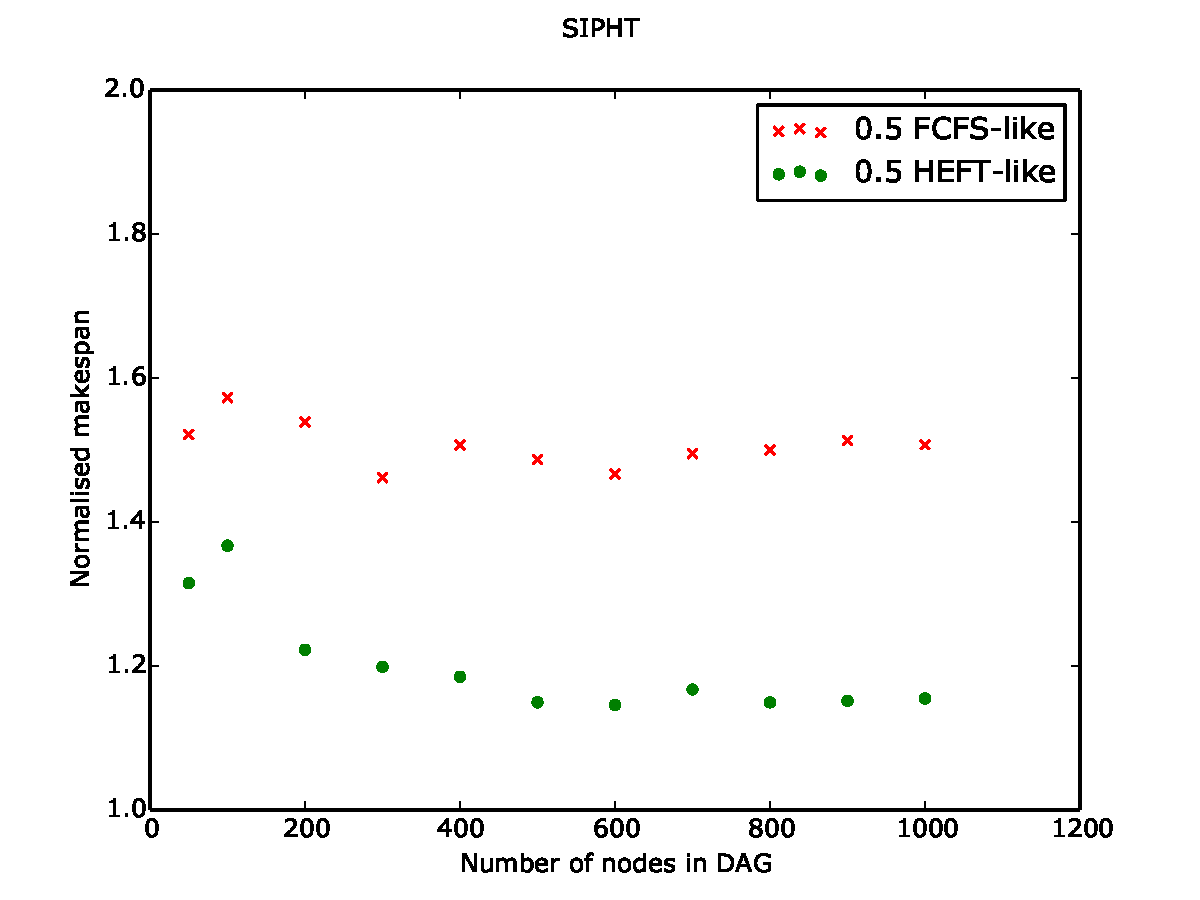
\includegraphics[width=\columnwidth]{{{images/schedule-length-ratio-SIPHT}}}
  \caption{\captionmacro{SIPHT}{\cite{Livny2008}}}
  \label{fig:sipht}
\end{figure}

\begin{figure}
  \centering
  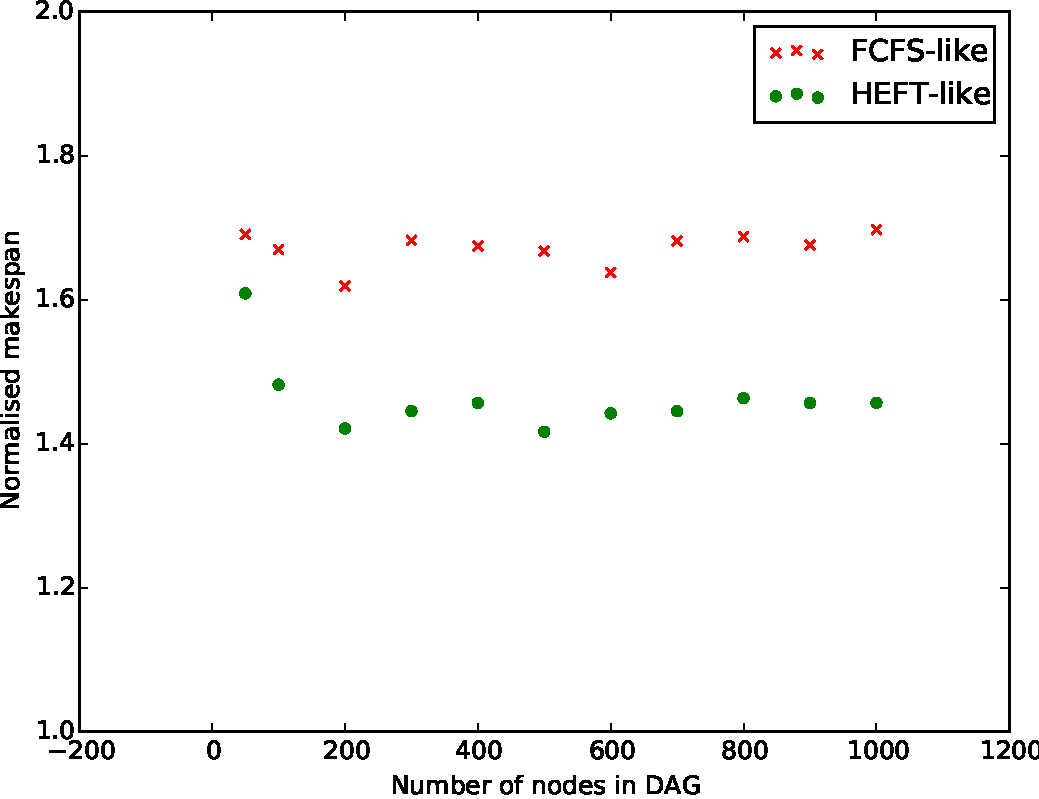
\includegraphics[width=\columnwidth]{{{images/schedule-length-ratio-GENOME}}}
  \caption{\captionmacro{GENOME}{\cite{epigenetics}}}
  \label{fig:genome}
\end{figure}

\section{Conclusion}

We have introduced an algorithm for resource provisioning and workflow scheduling under time-varying power constraints.
Our algorithm offers a reasonable improvement in the makespan over a naive dynamic scheduling approach.

\bibliographystyle{IEEEtran}
\bibliography{references}



\end{document}


